\documentclass[conference]{IEEEtran}
\usepackage{graphicx}
\usepackage{amsmath}
\usepackage{amssymb}
\usepackage{amsxtra}
\usepackage{amstext}
\usepackage{latexsym}
\usepackage{dsfont}
\usepackage{float}
\usepackage{cite}
\usepackage{subcaption}
\usepackage{epstopdf}
\usepackage{caption}
\ifCLASSINFOpdf
  % \usepackage[pdftex]{graphicx}
  % declare the path(s) where your graphic files are
  % \graphicspath{{../pdf/}{../jpeg/}}
  % and their extensions so you won't have to specify these with
  % every instance of \includegraphics
  % \DeclareGraphicsExtensions{.pdf,.jpeg,.png}
\else

\fi
\hyphenation{op-tical net-works semi-conduc-tor}
\begin{document}
\title{Influence of Polarization Direction on Static \\ On-Body Propagation Channels}
\author{Lingfeng~Liu$^1$, Peng~Zhang$^1$, Xiaonan~Wang$^1$, Chaoqun~Wang$^2$\\
\\
$^1$School of Information Engineering, East China Jiaotong University, China \\
$^2$School of Information Engineering, Nanchang University, China}
%\address{$^1$School of Information Engineering, East China Jiaotong University, China \\
%$^2$School of Information Engineering, East China Jiaotong University, China\\

%\small Email: Author@XXX.XXX
%}
\maketitle
\begin{abstract}
On-body propagation channels show significant polarization selectivity in static and dynamic scenarios. In this work, we measured polarized on-body channels on static body at 2.4 GHz by monopole antennas, where standing and sitting postures are considered. The polarization direction of the antenna ($Z$-polarization, $H$-polarization, $V$-polarization) depends on the direction of the antenna in the body position. In the statistical characteristics of the channels, the $V$-polarization direction of the receiving antenna is more conducive to receiving signal and reducing the path losses. Cross-polar discrimination (XPD) are calculated from measurement data, the strongly depolarization of on-body channels is more easily caused by the human sitting posture due to legs scattering. No matter how the polarization direction of the transmission antenna, the receiving antenna can generally obtain a decent field component in the $V$-polarization direction.
\end{abstract}
%\begin{keywords}

%\end{keywords}
%\IEEEpeerreviewmaketitle

%Check all references!!!!
%Check all references!!!!
%Check all references!!!!
%Check all references!!!!
%Check all references!!!!
%Check all references!!!!
%Check all references!!!!
\section{Introduction}
On-body communications in wireless body area networks (WBANs) are short distance communications (\textless\;2\;m) \cite{1} defined on or above the body of limited height. An essential feature of on-body propagation channels is that they do not follow conventional far-field propagation principles and exhibits complex near-field characteristics including the body scattering effects \cite{2} and surface wave propagation \cite{3}. Studies as \cite{4} have shown the high sensitivity of on-body channels to the orientation of the transmission and receiving antennas, implying the effectiveness of polarization diversity with a wearable BAN.

Earlier study on the finite-difference-time-domain (FDTD) simulations of the electromagnetic fields on the body surface \cite{manuscriptMap2017} has shown that due to the near-field body scattering effects, the surface wave propagation assumption may not fully consistent with the actual wave propagation in on-body channels, resulting the channel polarization dispersion both along and normal to the propagation path defined. The postures and body dynamics will further lead to the variation of the on-body polarization distribution over time and space domains. One limitation of previous measurements as reported in \cite{6,7,8} is that most of the measurements cover partial polarization combinations of on-body channels. Consequently, the polarization matrix of the channels are not fully characterized and modeled. Full-space description of the channel polarization distribution under specific scenarios is necessary to correctly capture the field components of the on-body channels.

In this work, measurements of polarized narrowband on-body channels at 2.4 GHz on static human body are conducted in indoor environment. Full polarization combinations are investigated for channels covering the key parts of the body. Two static postures of the body, i.e. the standing and sitting postures, were investigated, and the channel polarization distributions under the two postures were compared. The polarization matrix and the cross polarization discrimination (XPD) matrix for each scenario are summarized. The polarization gain and the depolarization ratio of the on-body channels are investigated.

This paper is organized as follows. Section \ref{sec:setup} describes the configuration of the measurements. Section \ref{sec:analysis} presents the statistical analysis of the channel polarization distribution and depolarization characteristics. Finally, Section \ref{sec:conclusion} summarizes the analysis.

\section{Measurement Settings}\label{sec:setup}

\begin{figure}[!t]
  \centering
  \begin{subfigure}[t]{0.3\textwidth}
  
\includegraphics[width=\textwidth]{figs/1a.eps}
  \caption{}
  \label{fig:volunteer}
  \end{subfigure}
  \begin{subfigure}[t]{0.25\textwidth}
  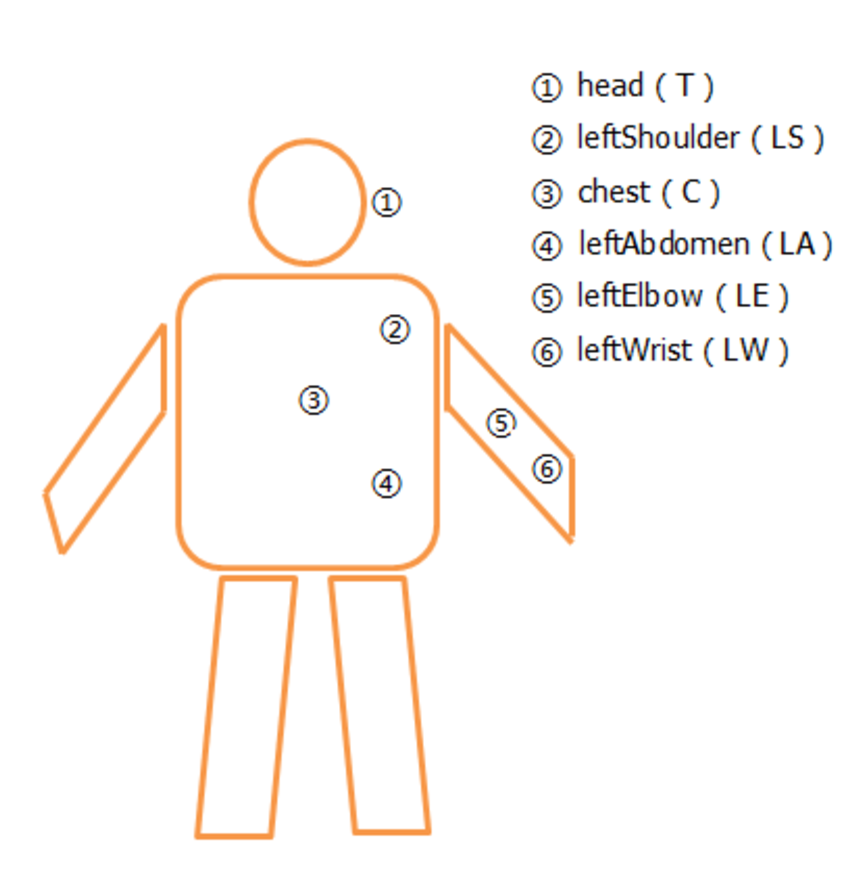
\includegraphics[width=4.5cm,height=5cm]{figs/1b.eps}
  \caption{}
  \label{fig:placement}
  \end{subfigure}
  \begin{subfigure}[t]{0.19\textwidth}
  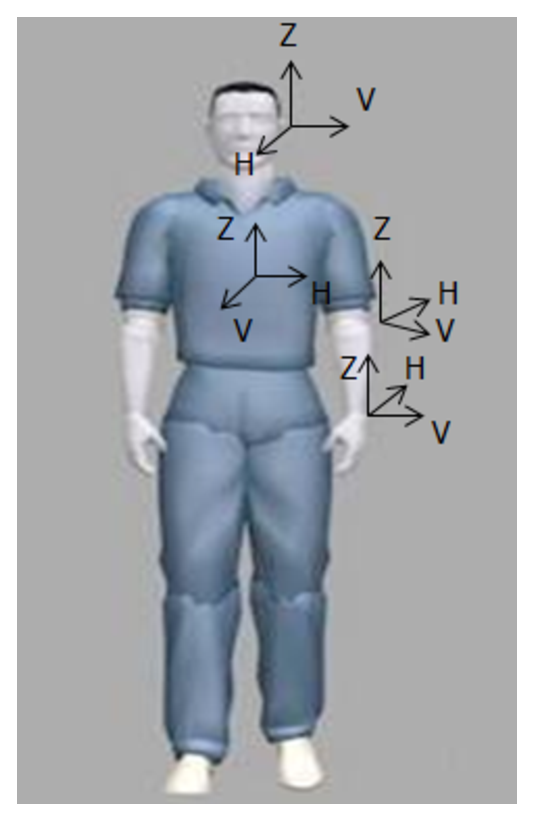
\includegraphics[width=3cm,height=5cm]{figs/1c.eps}
  \caption{}
  \label{fig:polarization_direction}
  \end{subfigure}
\caption{Measurement context at 2.4 GHz. (a) Indoor scenario and human body postures. (b) Node placement on the body. (c) The definition of Polarization direction in different parts of the body.}
\label{fig:human}
\end{figure}

The measurements were carried out in an indoor environment of an empty laboratory in dimension of 6 by 7 meters, no large obstacles around. We thereby assume the environment as reflection negligible, and on-body channels are primarily affected by their geometry distribution and body scattering.

A male volunteer of height 160 cm and weight 50 kg was chosen. Two postures, standing and sitting with arms naturally posed, are investigated as shown in Fig. \ref{fig:volunteer}. On-body channels were selected based on 5 key parts of the upper-body as presented in Fig. \ref{fig:placement}, which are head-left-shoulder (T-LS), head-left-wrist (T-LW), chest-left-abdomen (C-LA), left-shoulder-chest (LS-C), and left-elbow-left-wrist (LE-LW) channels. The ground reflection is also treated as minimized for these channels. Narrowband on-body channels at 2.4 GHz frequency band over time domain were measured on the body. To avoid heavy interference from the Wi-Fi signals, the actual frequency was selected at 2.484 GHz, i.e. an extra Wi-Fi channel not used in the China region.

A vector network analyzer (VNA) of type R\&S ZNB 20 was applied to measurement the channel S-parameters over time domain. The environment was quiet with no significant fading effects observed from the measurement. The analysis is then focused on the average channel loss. Monopole antennas of size 5 cm were used, mounted on the body 2 cm above the skin to alleviate the body coupling effects to the antenna efficiency. Setting details of the VNA and the antenna are presented in table \ref{tab:1}.

\begin{table}[!t]
\centering
\captionsetup{labelsep=newline}
\caption{Radio Settings}
\label{tab:1}
\begin{tabular}{cc}
\hline
Parameter&Value\\
\hline
VNA&ROHDE SCHWAR ZNB 20\\
Sampling points&1000\\
Transmit power&10 dBm\\
IF bandwidth&10 KHz\\
Sweep time&10 s\\
\hline
Antenna model&Monopole\\
Antenna size&5 cm\\
\hline
\end{tabular}
\end{table}


FDTD simulations as reported in \cite{} have shown that the field around the human body does not fully follow far-field propagation principles. The propagation path, as commonly defined by the surface wave presumption for on-body channels, may not be strictly perpendicular to the direction of the field polarization due to the body scattering effect and the near-field features of the radio waves. Consequently this will cause the polarization dispersion onto all directions. To effectively describe such inconsistency between the channel polarization and the propagation path, we suggest to define an on-body antenna's polarization in full-space dimension with respect to its relative positioning to the skin, which are vertical tangential, denoted as $Z$ direction, horizontal tangential, denoted as $H$ direction, and horizontal normal, denoted as $V$ direction, as denoted in Fig. \ref{fig:polarization_direction}. Note that because of the irregularity of the shapes of different parts of the body, the directions may be defined in different global orientations as well. By the extended definition of on-body antenna polarization, an on-body channel's polarization can be decomposed into 9 combinations, denoted as $XY$, $X, Y \in \{Z,V,H\}$, where $X$ is the polarization of the transmit antenna and $Y$ is the polarization of the receiving antenna.

\section{Measurement Statistical Analysis}\label{sec:analysis}

\begin{table}[!t]
\centering
\captionsetup{labelsep=newline}
\caption{Path Loss Summary of Measurements [dB]}
\label{tab:2}
\scalebox{0.85}{
\begin{tabular}{cccccccccc}
\hline
Standing &&&&&&&&&\\
Scenario&ZZ&ZV&ZH&VZ&VV&VH&HZ&HV&HH\\
\hline
T-LS&37.18&25.39&27.81&29.74&23.60&28.83&41.04&28.98&26.72\\
T-LW&58.11&37.21&47.69&59.12&42.78&61.49&61.84&48.39&62.10\\
C-LA&65.36&36.70&48.95&49.86&29.90&39.78&63.44&36.34&54.88\\
LS-C&50.38&30.32&43.70&49.68&30.69&54.65&54.81&35.68&45.71\\
LE-LW&47.66&23.92&31.12&42.14&29.99&29.93&50.10&30.33&27.97\\
\hline
\hline
Sitting &&&&&&&&&\\
Scenario&ZZ&ZV&ZH&VZ&VV&VH&HZ&HV&HH\\
\hline
T-LS&35.58&26.75&27.67&23.84&23.65&34.50&29.66&27.75&24.80\\
T-LW&53.47&39.17&39.60&58.62&47.17&46.49&58.22&39.24&43.51\\
C-LA&43.84&40.94&50.46&46.75&25.34&38.79&38.53&33.60&41.84\\
LS-C&47.02&30.60&48.15&50.81&31.09&50.89&45.27&36.66&46.30\\
LE-LW&39.05&35.77&32.07&44.11&28.52&32.32&56.16&33.52&25.91\\
\hline
\end{tabular}}
\end{table}


The average path losses of on-body channels in different polarization combinations are summarized in table \ref{tab:2} and categorized by the postures respectively.

\subsection{$V$-polarization convergence}

\begin{figure}[!t]
  \centering
  % Requires \usepackage{graphicx}
  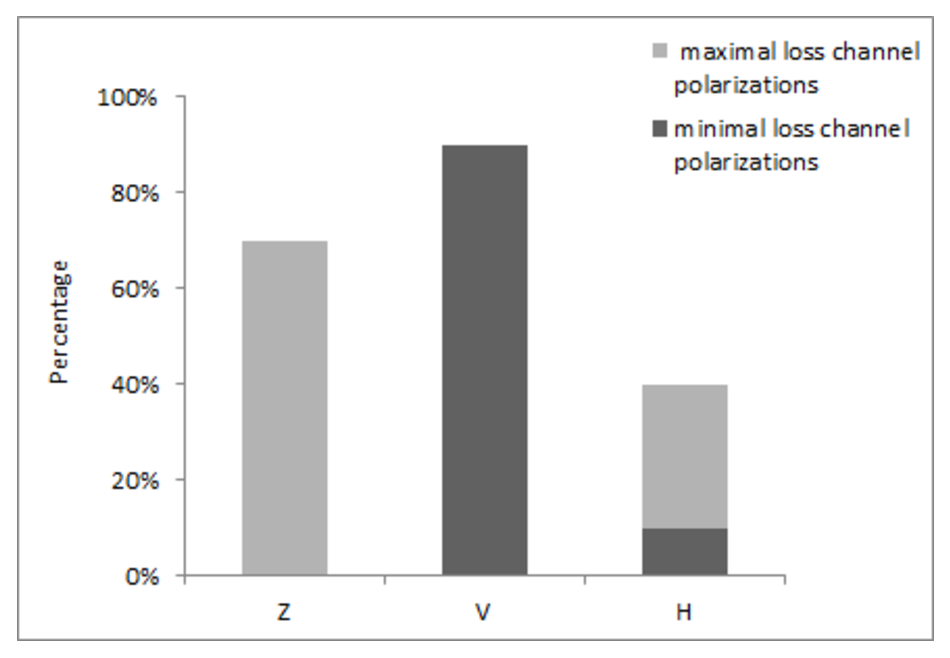
\includegraphics[width=0.4\textwidth]{figs/6.eps}\\
  \caption{The percentage of 3 polarizations of the receiving side in minimal loss channel polarizations and maximal loss channel polarizations respectively.}
  \label{fig:polarization percentage}
\end{figure}

The first observation of the channel loss in both postures is that most channels show $V$-polarization convergence at the receiving side. Under standing posture for instance, the minimal channel loss of scenarios T-LS and C-LA are achieved in $VV$ channel polarization, and $ZV$ channel polarization for T-LW, LS-C and LE-LW scenarios. Similar properties are also observed in these scenarios under the sitting posture. One exception under sitting postures is the LE-LW scenarios, whose minimal channel loss is achieved in $HH$ channel polarization, a possible consequence of the body coupling effect variation to the antennas during posture changes.

On the contrary, in all scenarios investigated in two postures, the maximal channel loss does not occur in channel polarizations with $V$-polarization at the receiving side for all polarizations at the transmit side.  In some scenarios, e.g. the T-LW and LS-C under sitting posture, the maximal channel loss is observed in channel polarization with $V$-polarization at the transmitting side instead of at the receiving side. As shown in Fig. \ref{fig:polarization percentage}, the percentage of $V$-polarization of the receiving side can up to 90 percent in minimal loss channel polarizations, $Z$-polarization at the receiving side should be avoided due to the proportion of up to 70 percent in maximal loss channel polarizations. This indicates that having the receiving antenna in $V$-polarization helps to capture the majority of the on-body channel field components.


The above observations show that on-body channels tend to have their field distributed along directions normal to the body. As consistent with previous FDTD simulations, the body coupling effect causes the absorbing of the on-body fields tangential to the skin, while the fields normal to the skin are less affected. As a result, the field will make the majority part along the normal direction. This may suggest therefore an optimal antenna emplacement for the communication aspects.

\subsection{Polarization gain}
\begin{figure}[!t]
  \centering
  % Requires \usepackage{graphicx}
  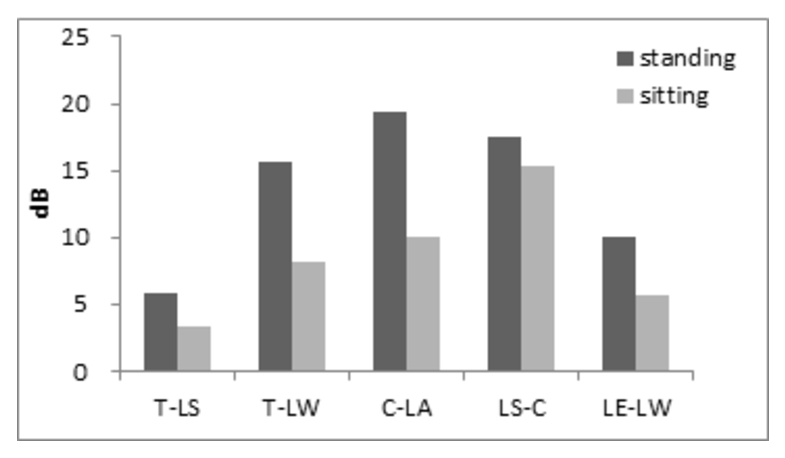
\includegraphics[width=0.4\textwidth]{figs/2.eps}\\
  \caption{The gain of receiving V-polarization of each channel in different postures.}
  \label{fig:2}
\end{figure}
\begin{figure*}[!t]
\centering
\begin{subfigure}[t]{\textwidth}
%\centerline{
\centering
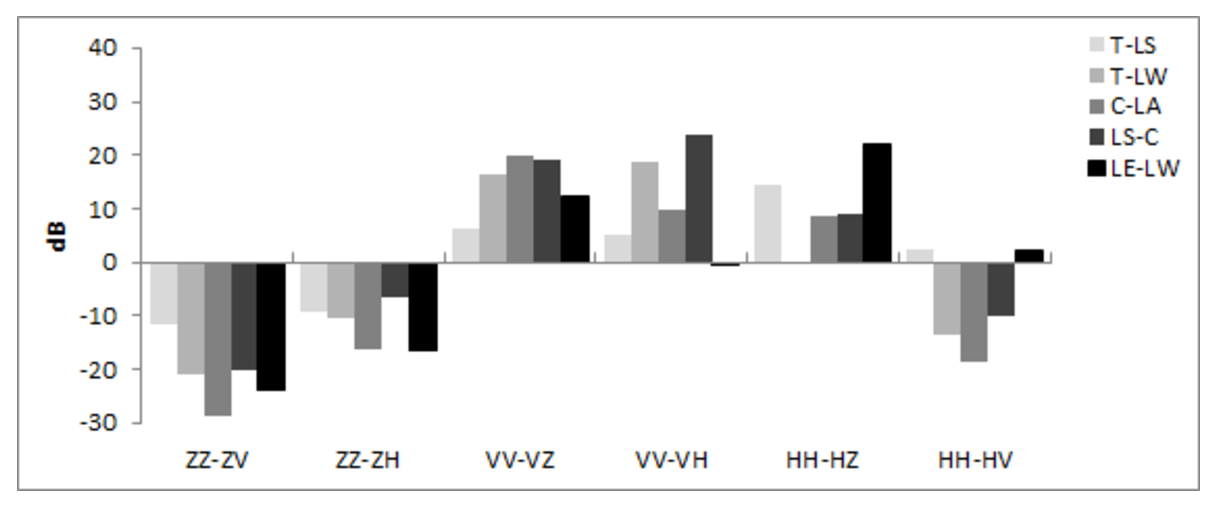
\includegraphics[width=14cm,height=4cm]{figs/3a.eps}
\subcaption{}
\label{fig:3a}
\end{subfigure}
\begin{subfigure}[t]{\textwidth}
\centering
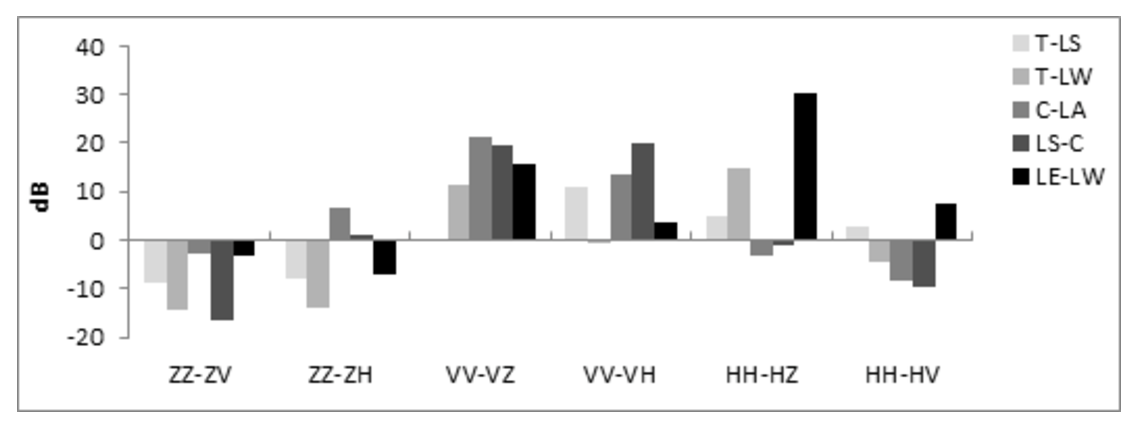
\includegraphics[width=14cm,height=4cm]{figs/3b.eps}
\subcaption{}
\label{fig:3b}
\end{subfigure}
\caption{XPD of on-body channels in six configurations. (a) XPD in the standing posture. (b) XPD in the sitting posture.}
\label{fig:3}
\end{figure*}

To quantize the receiving advantage of receiving $V$-polarization, we define its polarization gain in Eq. \ref{eq:1}.

\begin{equation}
	G_{V}=\frac{\sum\limits_I\sum\limits_J\text{PL}_{IJ}}{6} -\frac{\sum\limits_I{\text{PL}_{IV}}}{3},
\label{eq:1}
\end{equation}
where $I\in\{Z,H,V\}$ is the transmit polarization, $J\in\{Z,H\}$ is the receiving polarization other than $V$. $\text{PL}_{IJ}$ is the path loss of $IJ$ channel polarization, $\text{PL}_{IV}$ is the path loss of $IV$ channel polarization.

The $V$-polarization gain of each channel is summarized in Fig. \ref{fig:2}. In general, the $V$-polarization gain of scenarios under standing posture is better than that under sitting posture. The $V$-polarization gain of scenarios under standing posture is in average greater than 5 dB. Meanwhile, $V$-polarization gain of scenarios under sitting posture is in average greater than 3 dB.

\subsection{Channel depolarization}
The results presented in table \ref{tab:2} show as well heavy cross polarization in different scenarios. If the on-body communication systems are designed following regular antenna emplacement, i.e. the orientation of the antennas are either in $Z$, $H$, or $V$ directions, such cross polarization may cause the actual field polarization of the on-body channel be apart from these regular directions. We denote this as the channel depolarization effect.

The channel depolarization can be described via the cross-polarization discrimination (XPD), calculated by Eq. \ref{eq:2}.

 \begin{align}
	 \text{XPD}_{i,j}&=\frac{P_{ii}}{P_{ij}} \quad[dB]\nonumber\\
	 &=\text{PL}_{ij}[dB]-\text{PL}_{ij}[dB], \label{eq:2}
\end{align}
where $i,j \in \{V,H,Z\}$, $P_{ii}$ is the power of the co-polarized channel component and $P_{ij}$ is the cross-polarized channel component.

The XPD in Eq. \ref{eq:2} may describe three situations of the channel cross-polarization. First, if XPD is positive, the higher of the value indicates that the channel tends to concentrate on its co-polarization component. Second, if XPD is negative, the smaller of the value indicates that the channel is transmitting its fields to the cross-polarization component. Third, if the absolute XPD is less than 10 dB, the channel is considered to be depolarized, and the value gets close to 0 dB, the field will be projected both onto the co-polarized and cross-polarized components of the channel.

%Complete the symbols!!!!!!!!!!!!!!!!!
%Complete the symbols!!!!!!!!!!!!!!!!!
%Complete the symbols!!!!!!!!!!!!!!!!!
%Complete the symbols!!!!!!!!!!!!!!!!!

We studied in total of 6 XPD configurations in the investigated channels, which are $\text{XPD}_{Z,V}$, $\text{XPD}_{Z,H}$, $\text{XPD}_{V,Z}$, $\text{XPD}_{V,H}$, $\text{XPD}_{H,Z}$, $\text{XPD}_{H,V}$, as presented in Fig. \ref{fig:3}, categorized in two postures.

%Define |XPD| < 10 dB can be viewed as channel containing depolarization
%Define |XPD| < 10 dB can be viewed as channel containing depolarization
%Define |XPD| < 10 dB can be viewed as channel containing depolarization
%Define |XPD| < 10 dB can be viewed as channel containing depolarization

As shown as the Fig. \ref{fig:3}(a), the negative values of $\text{XPD}_{Z,V}$ and $\text{XPD}_{Z,H}$ configurations show the cross-polarized configuration remain dominant in all channels, and $ZV$ combination is better suited to on-body channels than $ZH$ combination because of the larger absolute $\text{XPD}_{Z,V}$. The positive values of $\text{XPD}_{V,Z}$ configuration show $VV$ combination remains dominate in each channel. On the other hand, the LE-LW channel is strongly depolarized in $\text{XPD}_{V,H}$ and $\text{XPD}_{H,V}$ configurations, with the XPD close to 0 dB. The strong depolarization also occurred in T-LW channel of $\text{XPD}_{H,Z}$ configuration and T-LS channel of $\text{XPD}_{H,V}$ configuration. The XPD of the sitting posture is shown in Fig. \ref{fig:3}(b). We can find that the phenomenon of depolarization is more common. On-body channels of $\text{XPD}_{Z,H}$ and $\text{XPD}_{H,V}$ configurations are generally depolarized, where most of the absolute values are less 10 dB or even close to 0 dB. The channel depolarization also occurred in other configurations, for example, C-LA channel in $\text{XPD}_{Z,V}$ configuration and T-LS channel in $\text{XPD}_{V,H}$ configuration. These show human sitting posture is more likely to cause depolarization of on-body channels.

In addition to individual cases mentioned above, since the absolute values of each configuration are nearly equal to 10 dB or more for most on-body channels, most channels of all kinds of configurations can keep a stable polarization characteristic in the standing posture. Unlike the case of  the standing posture, we can find that the number of channels with stable polarization characteristic in each scenario is significantly reduced under the sitting posture, especially in the case of configurations $\text{XPD}_{Z,V}$ and $\text{XPD}_{Z,H}$. The main reason is that on-body channels are affected by the leg scattering, while the placement of the arm also will cause certain interference to the on-body communication links in the sitting posture.

%1. paragraph on cross polarization (xpd>10 db)
%2. paragraph on depolarization (xpd < 10 db)

Besides, we find that the values of the on-body propagation channels under the configurations $\text{XPD}_{Z,V}$ and $\text{XPD}_{H,V}$ are generally negative, while the $\text{XPD}_{V,Z}$ and $\text{XPD}_{V,H}$ configurations are generally positive values, regardless of the standing and sitting postures. These indicate that the receiving antenna can generally obtain the decent component of the field in the $V$-polarization direction, regardless of the polarization direction polarization of the transmission antenna. At the same time, this is also the reason why the receiving antenna with $V$-polarization can effectively receive signal and reduce the path loss.

\section{Conclusion}\label{sec:conclusion}
In this paper, measurement results of narrowband polarized static on-body channels at 2.4 GHz are presented under complete polarization combination in space. Analyses of the measurements demonstrate that $V$-polarization of the receiving antenna can effectively reduce the path loss and capture signal waves. The gain of receiving $V$-polarization of each channel can up to at least 3 dB in the sitting posture, the $V$-polarization gain of each on-body channel can up to at last 5 dB in the standing posture. Depolarization of on-body channels is more serious in the sitting posture due to the effect of leg scattering. The receiving antenna with $V$-polarization is more beneficial to obtain the decent field component compared with the $Z$ and $H$ polarization of the receiving antenna by analyzing the depolarization characteristics of static on-body channels, regardless of the polarization direction of the transmission antenna. This once again proved that the receiving antenna with $V$-polarization can effectively reduce the path loss.

\section*{Acknowledgment}
This paper was supported by the Natural Science Foundation of China (NSFC) under grant No.81460275.

\begin{thebibliography}{1}

\bibitem{1}
Bae, Joonsung, and Hoi-Jun Yoo. "The effects of electrode configuration on body channel communication based on analysis of vertical and horizontal electric dipoles." \emph{IEEE Transactions on Microwave Theory and Techniques} 63.4 (2015): 1409-1420.
%H.~Kopka and P.~W. Daly, \emph{A Guide to \LaTeX}, 3rd~ed.\hskip 1em plus
  %0.5em minus 0.4em\relax Harlow, England: Addison-Wesley, 1999.
\bibitem{2}
Lu, Xiyu, et al. "UWB-based Wireless Body Area Networks channel modeling and performance evaluation." \emph{Wireless Communications and Mobile Computing Conference (IWCMC), 2011 7th International.} IEEE, 2011.
%Li, Yang, et al. "Human Activity Classification Based on Dynamic Time Warping of an On-Body Creeping Wave Signal." \emph{IEEE Transactions on Antennas and Propagation} 64.11 (2016): 4901-4905.
\bibitem{3}
Li, Yang, et al. "Human Activity Classification Based on Dynamic Time Warping of an On-Body Creeping Wave Signal." \emph{IEEE Transactions on Antennas and Propagation} 64.11 (2016): 4901-4905.
%Kumpuniemi, Timo, et al. "Dynamic on-body UWB radio channel modeling." \emph{Medical Information and Communication Technology (ISMICT), 2015 9th International Symposium on}. IEEE, 2015.
\bibitem{4}
Aoyagi, Takahiro, et al. "Numerical simulations for dynamic WBAN propagation channel during various human movements." \emph{Medical Information $\&$ Communication Technology (ISMICT), 2011 5th International Symposium on.} IEEE, 2011.
\bibitem{manuscriptMap2017}
L. Liu, X. Wang, and N. Jiang. "Investigation of on-body channel polarization distribution around the torso at 2.45 GHz by FDTD simulations." \emph{submitted to IET MAP.} 2017
\bibitem{6}
Li, Kun, Kazuhiro Honda, and Koichi Ogawa. "Analysis of the body proximity cross-polarization power ratio in a human walking motion." \emph{Microwave Conference (APMC), 2015 Asia-Pacific.} Vol. 2. IEEE, 2015.
%Uusitupa, Tero, and Takahiro Aoyagi. "Analysis of dynamic on-body communication channels for various movements and polarization schemes at 2.45 GHz." \emph{IEEE Transactions on Antennas and Propagation} 61.12 (2013): 6168-6179.
\bibitem{7}
Petrillo, Luca, et al. "Statistical on-body measurement results at 60 GHz." \emph{IEEE transactions on antennas and propagation} 63.1 (2015): 400-403.
%Paraskevopoulos, A., et al. "Modelling of dynamic on-body channels using different types of wearable antennas." \emph{Antennas and Propagation (EuCAP)}, 2014 8th European Conference on. IEEE, 2014.
\bibitem{8}
Nechayev Y I, Constantinou C C, Wu X, et al. De-polarization of on-body channels and polarization diversity at 60 GHz[J]. \emph{IEEE Transactions on Antennas and Propagation,} 2014, 62(12): 6519-6523.
%\bibitem{10}
%Aoyagi, Takahiro, et al. "Numerical simulations for dynamic WBAN propagation channel during various human movements." \emph{Medical Information & Communication Technology (ISMICT), 2011 5th International Symposium on.} IEEE, 2011.
%\bibitem{11}
%Lu, Xiyu, et al. "UWB-based Wireless Body Area Networks channel modeling and performance evaluation." \emph{Wireless Communications and Mobile Computing Conference (IWCMC), 2011 7th International.} IEEE, 2011.
\end{thebibliography}




% that's all folks
\end{document}
